\documentclass[12pt,]{article}
\usepackage{lmodern}
\usepackage{amssymb,amsmath}
\usepackage{ifxetex,ifluatex}
\usepackage{fixltx2e} % provides \textsubscript
\ifnum 0\ifxetex 1\fi\ifluatex 1\fi=0 % if pdftex
  \usepackage[T1]{fontenc}
  \usepackage[utf8]{inputenc}
\else % if luatex or xelatex
  \ifxetex
    \usepackage{mathspec}
  \else
    \usepackage{fontspec}
  \fi
  \defaultfontfeatures{Ligatures=TeX,Scale=MatchLowercase}
\fi
% use upquote if available, for straight quotes in verbatim environments
\IfFileExists{upquote.sty}{\usepackage{upquote}}{}
% use microtype if available
\IfFileExists{microtype.sty}{%
\usepackage{microtype}
\UseMicrotypeSet[protrusion]{basicmath} % disable protrusion for tt fonts
}{}
\usepackage[margin=1in]{geometry}
\usepackage{hyperref}
\hypersetup{unicode=true,
            pdftitle={Algorithmic Approaches to Match Degraded Land Impressions},
            pdfauthor={Eric Hare, Heike Hofmann, Alicia Carriquiry},
            pdfborder={0 0 0},
            breaklinks=true}
\urlstyle{same}  % don't use monospace font for urls
\usepackage{longtable,booktabs}
\usepackage{graphicx,grffile}
\makeatletter
\def\maxwidth{\ifdim\Gin@nat@width>\linewidth\linewidth\else\Gin@nat@width\fi}
\def\maxheight{\ifdim\Gin@nat@height>\textheight\textheight\else\Gin@nat@height\fi}
\makeatother
% Scale images if necessary, so that they will not overflow the page
% margins by default, and it is still possible to overwrite the defaults
% using explicit options in \includegraphics[width, height, ...]{}
\setkeys{Gin}{width=\maxwidth,height=\maxheight,keepaspectratio}
\IfFileExists{parskip.sty}{%
\usepackage{parskip}
}{% else
\setlength{\parindent}{0pt}
\setlength{\parskip}{6pt plus 2pt minus 1pt}
}
\setlength{\emergencystretch}{3em}  % prevent overfull lines
\providecommand{\tightlist}{%
  \setlength{\itemsep}{0pt}\setlength{\parskip}{0pt}}
\setcounter{secnumdepth}{5}
% Redefines (sub)paragraphs to behave more like sections
\ifx\paragraph\undefined\else
\let\oldparagraph\paragraph
\renewcommand{\paragraph}[1]{\oldparagraph{#1}\mbox{}}
\fi
\ifx\subparagraph\undefined\else
\let\oldsubparagraph\subparagraph
\renewcommand{\subparagraph}[1]{\oldsubparagraph{#1}\mbox{}}
\fi

%%% Use protect on footnotes to avoid problems with footnotes in titles
\let\rmarkdownfootnote\footnote%
\def\footnote{\protect\rmarkdownfootnote}

%%% Change title format to be more compact
\usepackage{titling}

% Create subtitle command for use in maketitle
\newcommand{\subtitle}[1]{
  \posttitle{
    \begin{center}\large#1\end{center}
    }
}

\setlength{\droptitle}{-2em}
  \title{Algorithmic Approaches to Match Degraded Land Impressions}
  \pretitle{\vspace{\droptitle}\centering\huge}
  \posttitle{\par}
  \author{Eric Hare, Heike Hofmann, Alicia Carriquiry}
  \preauthor{\centering\large\emph}
  \postauthor{\par}
  \predate{\centering\large\emph}
  \postdate{\par}
  \date{9/5/2017}

\usepackage{float}

\usepackage{amsthm}
\newtheorem{theorem}{Theorem}[section]
\newtheorem{lemma}{Lemma}[section]
\theoremstyle{definition}
\newtheorem{definition}{Definition}[section]
\newtheorem{corollary}{Corollary}[section]
\newtheorem{proposition}{Proposition}[section]
\theoremstyle{definition}
\newtheorem{example}{Example}[section]
\theoremstyle{definition}
\newtheorem{exercise}{Exercise}[section]
\theoremstyle{remark}
\newtheorem*{remark}{Remark}
\newtheorem*{solution}{Solution}
\begin{document}
\maketitle

\textbf{Abstract}

Bullet matching is a process used to determine whether two bullets may
have been fired from the same gun barrel. Historically, this has been a
manual process performed by trained forensic examiners. Recent work
however has shown that it is possible to add statistical validity and
objectivity to the procedure. In this paper, we build upon the
algorithms explored in Automatic Matching of Bullet Lands (Hare,
Hofmann, and Carriquiry 2016) by formalizing and defining a set of
features, computed on pairs of bullet lands, which can be used in
machine learning models to assess the probability of a match. We then
use these features to perform an analysis of the two Hamby (Hamby,
Brundage, and Thorpe 2009) bullet sets (Set 252 and Set 44), to assess
the presence of microscope operator effects in scanning. We also take
some first steps to address the issue of degraded bullet lands, and
provide a range of degradation at which the matching algorithm still
performs well. Finally, we discuss generalizing land to land comparisons
to full bullet comparisons as would be used for this procedure in a
criminal justice situation.

\section{Background}\label{background}

Intense scrutiny has been focused on the process of bullet matching in
recent years (e.g., Giannelli 2011). Bullet matching, the process of
determining whether two bullets could have been fired from the same gun
barrel, has traditionally been performed without meaningful
determination of error rates or statistical assessments of uncertainty
(National Research Council 2009). There have been some attempts towards
developing mathematical and statistical approaches to bullet
matching.One such attempt was the definition of CMS, the Consecutively
Matching Striae (Biasotti 1959), with a cutoff of six to separate
matches from non-matches. Still, rigorous assessments of the
applicability of such cutoffs have not to this point been described
(Advisors on Science and Technology 2016).

Recently, several authors have addressed these well-known shortcomings.
Focusing on firing pin impressions and breech faces, Riva and Champod
(2014) have described an automated algorithm using 3D images that
enables comparison between pairs of exemplars. Other examples of work in
this and related areas include Petraco and Chan (2012), W. Chu et al.
(2011), T. Vorburger et al. (2011), and others. In our approach to this
problem, Automatic Matching of Bullet Lands, we used the Hamby 252 set
(Hamby, Brundage, and Thorpe 2009) to train and develop a random forest
in order to provide a matching probability for two bullet lands (Hare,
Hofmann, and Carriquiry 2016). While the algorithm had a very strong
performance on this set, some limitations were immediately clear. For
instance, performance was assessed only on this single set of 35 bullets
fired from a consecutively manufactured set of only ten gun barrels.
Each of these bullets was part of controlled study, and the full lands
were available for matching. While there were some data quality issues,
this was still a near ideal test case for the algorithm.

Real world applications of bullet matching often involve the recovery of
fragments of bullets from the crime scene. Traditional features used in
forensic examination work well for a full land, but there has been less
investigation into their performance in the case of a fragmented land.
For example, the CMS is naturally limited by the portion of the land
that can be recovered.

In this paper, we take steps to address these and other concerns.
Specifically, we begin by reviewing features from the literature,
computed on pairs of bullet lands, and presenting some of our own
features. We propose an approach to standardize the featues, to account
for the fact that only a portion of the land impression may be recovered
from the crime scene. With the standardized features, we tackle two
issues that were not addressed in (Hare, Hofmann, and Carriquiry 2016).
The first is the effect of the microscope operator on the resulting
images and consequent algorithm performance. The second issue has to do
with the robustness of the land matching algorithm in (Hare, Hofmann,
and Carriquiry 2016) relative to the degree of degradation of the
questioned land impression. Finally, we describe some of the initial
steps toward generalizing a matching algorithm based on land-to-land
comparisons, to one based on bullet-to-bullet comparisons, as would be
of interest in a real world application of these ideas.

\section{Feature Standardization}\label{feature-standardization}

To start, we introduce a standardized version of each of the features
used in the matching routine proposed by (Hare, Hofmann, and Carriquiry
2016). These features are computed on \emph{aligned pairs of bullet land
impressions} rather than on individual lands. This enables us, for
instance, to compute the number of matching striae. Table \ref{tab:ccf1}
and Table \ref{tab:ccf2} provide an example of six land-to-land
comparisons and the derived features for these comparisons. The two
\texttt{profile\_id} columns identify a particular land from the two
Hamby datasets, and the remaining columns are the derived features for
these comparisons.

\begin{table}[ht]
\centering
\begin{tabular}{rrrrrrr}
  \hline
profile1\_id & profile2\_id & ccf & rough\_cor & lag & D & sd\_D \\ 
  \hline
49 & 540 & 0.2689 & 0.1091 & -0.1734 & 0.0026 & 0.0043 \\ 
  49 & 1032 & 0.3878 & 0.3582 & 0.1938 & 0.0017 & 0.0030 \\ 
  49 & 1540 & 0.2410 & 0.1320 & 0.2781 & 0.0023 & 0.0039 \\ 
  49 & 2044 & 0.2892 & 0.1136 & 0.0828 & 0.0023 & 0.0038 \\ 
  49 & 2583 & 0.1769 & 0.0214 & -0.0563 & 0.0026 & 0.0041 \\ 
  49 & 3074 & 0.2715 & 0.1254 & 0.0938 & 0.0020 & 0.0033 \\ 
   \hline
\end{tabular}
\caption{A sample of six land-to-land comparisons, and derived features for these comparisons.} 
\label{tab:ccf1}
\end{table}

\begin{table}[ht]
\centering
\begin{tabular}{rrrrrrr}
  \hline
signature\_length & overlap & matches & mismatches & cms & non\_cms & sum\_peaks \\ 
  \hline
1.9328 & 0.9103 & 1.1368 & 10.2251 & 0.5684 & 3.7182 & 2.0038 \\ 
  1.9359 & 0.9193 & 5.0571 & 6.5593 & 3.3714 & 2.3426 & 6.5264 \\ 
  1.9359 & 0.8757 & 1.7696 & 10.3662 & 1.1797 & 5.8592 & 2.0192 \\ 
  1.9172 & 0.9829 & 1.5920 & 7.9441 & 0.5307 & 3.4756 & 1.8139 \\ 
  1.8234 & 0.9692 & 1.1317 & 8.8479 & 0.5659 & 4.9155 & 0.8555 \\ 
  1.9172 & 0.9690 & 2.6913 & 10.7645 & 1.0765 & 3.4251 & 3.5272 \\ 
   \hline
\end{tabular}
\caption{The remaining derived features for the previous six land-to-land comparisons.} 
\label{tab:ccf2}
\end{table}

We generalize the definitions of these features to account for the
possibility that we may be handling degraded bullet lands, where only
fragments can be recovered. The definition of each feature is given
below, where \(f(t)\) represents the height values of the first profile,
and \(g(t)\) the height values of the second:

\begin{itemize}
\tightlist
\item
  \textbf{ccf} (\%) is the maximum value of the Cross-Correlation
  function evaluated at the optimal alignment. The Cross-Correlation
  function is defined as
  \(C(\tau) = \int_{-\infty}^{\infty} f(t)g(t + \tau)dt\) where \(\tau\)
  represents the the lag of the second signature (T. Vorburger et al.
  2011).
\item
  \textbf{rough\_cor} (\%) is a new feature that quantifies the
  correlation between the two signatures after performing a second LOESS
  smoothing stage and then subtracting the result from the original
  signatures. This attempts to model the roughness of the surface after
  removing structure such as waviness.
\item
  \textbf{lag} (mm) Is the optimal lag for the ccf value.
\item
  \textbf{D} (mm) is the Euclidean vertical distance between each height
  value of the aligned signatures. This is defined as
  \(D^2 = \frac{1}{\text{\#}t}\sum_t \left[f(t) - g(t)\right]^2\). This
  is a measure of the total variation between two functions (Clarkson
  and Adams 1933).
\item
  \textbf{sd\_D} (mm) provides the standard deviation of the values of
  \emph{D} from above.
\item
  \textbf{signature\_length} (mm) is the overall length of the smallest
  of the two aligned signatures.
\item
  \textbf{overlap} (\%) provides the percentage of the two signatures
  that overlap after the alignment stage.
\item
  \textbf{matches} (per mm) is the number of matching peaks/valleys
  (striae) per millimeter of the overlapping portion of the aligned
  signatures.
\item
  \textbf{mismatches} (per mm) is the number of mismatching
  peaks/valleys (striae) per millimeter of the overlapping portion of
  the aligned signatures.
\item
  \textbf{cms} (per mm) is the number of consecutively matching
  peaks/valleys (striae) per millimeter of the overlapping portion of
  the aligned signatures (Biasotti 1959, Wei Chu et al. (2013)).
\item
  \textbf{non\_cms} (per mm) is the number of consecutive mismatching
  peaks/valleys (striae) per millimeter of the overlapping portion of
  the aligned signatures.
\item
  \textbf{sum\_peaks} (per mm) is the the sum of the average heights of
  matched striae.
\end{itemize}

The features that are expressed on a per millimeter level are intended
to support the degraded land case, as discussed earlier. Note that the
computation differs slightly depending on the feature. For example, to
standardize the number of matches, the first count the raw number of
matching striae, and then divide this number by the length of the
overlapping region of the two lands (\texttt{overlap} from above). In
most cases, the overlapping region will be very close to the length of
the smaller signature. But depending on the alignment, this may not
always be true. This ensures that we do not punish a particular
cross-comparison for having a smaller region in which matches could
occur. On the other hand, the number of mismatches is divided by the
total length of the two aligned signatures, since mismatched striae can
occur even in the non-overlapping region of the two signatures.

The \texttt{rough\_cor} or Roughness Correlation is derived by
performing a second smoothing step, and subtracting the result from the
original signatures. This creates a new signature which eliminates some
of the overall structure, allowing global deformations to have less of
an influence on the model output. Where the roughness correlation is
most useful is in a scenario like Figure \ref{fig:roughcorgood}. This
figure shows the alignment of profile 40977 with 47600. The top panel
shows the smoothed signatures. The middle panel overlays a LOESS fit to
the average of the two signatures. Finally, to derive the roughness
correlation, this LOESS is subtracted from the original signature to
create a new set of roughness residuals, which are then given in the
bottom panel. Note that these two profiles do not match, yet the ccf is
0.7724. The roughness correlation (-0.0324) correctly indicates the lack
of matching. The roughness correlation acts as a check against false
positives which can arise when there are significant deformations in the
overall structure, as in the case with both these profiles.

\begin{figure}[htbp]
\centering
\includegraphics{degraded-paper_files/figure-latex/roughcorgood-1.pdf}
\caption{\label{fig:roughcorgood}Alignment of profile 40977 with 47600. The
top panel shows the smoothed signatures. The middle panel overlays a
LOESS fit to the average of the two signatures. Finally, to derive the
roughness correlation, this LOESS is subtracted from the original
signature to create a new set of roughness residuals, which are then
given in the bottom panel. Note that these two profiles do not match,
yet the ccf is 0.7724. The roughness correlation (-0.0324) correctly
indicates the lack of matching.}
\end{figure}

In a typical comparison between two profiles, such as in Figure
\ref{fig:roughcorfine}, the roughness correlation does not meaningfully
impact the matching probability given the presence of the ccf in the
model. In this figure, we see the alignment of profile 8752 with profile
136676. In this case, the waviness or the deformation pattern in the
signatures is less pronounced, and hence the resulting roughness
signature resembles the original signature more closely. These profiles
match, and both ccf (0.6891) and rough\_cor (0.7980) provide values
indicative of matching.

\begin{figure}[htbp]
\centering
\includegraphics{degraded-paper_files/figure-latex/roughcorfine-1.pdf}
\caption{\label{fig:roughcorfine}Alignment of profile 8752 with profile
136676. In this case, the waviness or the deformation pattern in the
signatures is more minor, and hence the resulting roughness signature
resembles the original signature more closely. These profiles match, and
both ccf (0.6891) and rough\_cor (0.7980) provide values indicative of
matching.}
\end{figure}

We can observe the distributions of both CCF and the Roughness
Correlation side by side, differentiating between known matches and
known non-matches. Figure \ref{fig:roughcordist} shows this. It can be
seen that the separation of the two groups along both variables is quite
strong, but many known-matches have low values for each. The
distributions of known non-matches, on the other hand, is relatively
symmetric and normal.

\begin{figure}[htbp]
\centering
\includegraphics{degraded-paper_files/figure-latex/roughcordist-1.pdf}
\caption{\label{fig:roughcordist}Distributions of the Roughness Correlation
compared to the CCF for known matches and known non-matches}
\end{figure}

\section{Model Training}\label{model-training}

Using these features, we can train a randomForest (Liaw and Wiener 2002)
model which attempts to predict whether two lands match given the value
of the features. There are currently three studies for bullets included
in the NIST ballistics database (REF). Those are Hamby (Set 252), Hamby
(Set 44), and Cary. For purposes of analysis we describe in this paper,
we exclude the Cary bullets from consideration, because the study was
designed to assess the persistence of striation markings over a series
of fires from the same barrel. Thus, every Cary bullet is a known match
to every other Cary bullet, although early firings do not produce the
same markings that later firings do. Hence, we will consider Hamby (Set
252) and Hamby (Set 44) only.

We can now train the forest using the features we defined earlier. We
split the data into an 80\% training, 20\% testing sets to assess the
algorithm's out of sample performance, using the \texttt{caret} package
(Jed Wing et al. 2016). Table \ref{tab:avgforest} displays the results
in the form of a confusion matrix on the test set, averaged over ten
independent random forests trained on ten random data subsets. There are
a total of 83,028 land-to-land comparisons, of which 1208 are among
known matching land impressions and 81,820 are among known non-matching
land impressions. It can be seen that false positives are exceedingly
rare, but false negatives occur more frequently (approximately 65 false
negative land to land comparisons on the test set, compared with an
average of less than four false positives).

\begin{table}[H]
\centering
\begin{tabular}{lr}
  \hline
Result & Count \\ 
  \hline
False Negative & 65.3 \\ 
  False Positive & 3.8 \\ 
  True Negative & 16363.1 \\ 
  True Positive & 171.8 \\ 
   \hline
\end{tabular}
\caption{The average confusion matrix for the 10 random forests. It can be seen that false positives are exceedingly rare, but false negatives occur more frequently.} 
\label{tab:avgforest}
\end{table}

These results suggest that our algorithm is too conservative in
predicting a match when in fact the bullets were fired from the same gun
barrel. We can break down the confusion matrix by the study from which
each of the two land impressions originated. Table
\ref{tab:avgforeststudy} shows the average confusion matrix for the 10
random forests, broken down by study. It can be seen that Hamby252 to
Hamby252 comparisons exhibit the fewest errors, while Hamby252 to
Hamby44 comparisons exhibit the most errors on average. This intuitively
makes some sense given the potential presence of scanner operator
effects, which we address further in this section.

\begin{table}[H]
\centering
\begin{tabular}{lllll}
  \hline
Study & False Negative & False Positive & True Negative & True Positive \\ 
  \hline
Hamby252\_Hamby252 & 0.29\% & 0.01\% & 98.77\% & 0.93\% \\ 
  Hamby252\_Hamby44 & 0.47\% & 0.02\% & 98.35\% & 1.16\% \\ 
  Hamby44\_Hamby44 & 0.34\% & 0.04\% & 98.72\% & 0.9\% \\ 
   \hline
\end{tabular}
\caption{The average confusion matrix for the 10 random forests, broken down by study. It can be seen that Hamby252 to Hamby252 comparisons exhibit the fewest errors, while Hamby252 to Hamby44 comparisons exhibit the most on average.} 
\label{tab:avgforeststudy}
\end{table}

\section{Feature Robustness}\label{feature-robustness}

As a first stage to assessing feature robustness, we produce parallel
coordinate plots of the various features based on true positives, true
negatives, false positives, and false negatives. Figures \ref{fig:pcp}
and \ref{fig:pcp2} display these plots. The means of the true positive
and the false negative groups are shown, respectively, in the two
figures. False positives tend to occur with anomalously high values of
\texttt{sum\_peaks}, \texttt{matches}, and \texttt{ccf}, while false
negatives tend to resemble very closely the feature distribution of the
true negatives, with a slightly higher average \texttt{ccf}.

\begin{figure}[htbp]
\centering
\includegraphics{degraded-paper_files/figure-latex/pcp-1.pdf}
\caption{\label{fig:pcp}Parallel coordinate plot of the features based on
the random forest confusion matrix for true and false positives.}
\end{figure}

\begin{figure}[htbp]
\centering
\includegraphics{degraded-paper_files/figure-latex/pcp2-1.pdf}
\caption{\label{fig:pcp2}Parallel coordinate plot of the features based on
the random forest confusion matrix for true and false negatives.}
\end{figure}

\subsection{Operator Effects}\label{operator-effects}

We attempt to quantify the effect of the study on the matching
probability by fitting a new random forest which is designed to predict
the study based on the derived features. Ideally, if the assumption of
independence between lands holds across different operators, this forest
should have poor performance - The set of derived features should be
relatively consistent among known matches and known non-matches
regardless of the study since the Hamby data in both sets originated
from the same gun barrels.

Table \ref{tab:studypred} shows the confusion matrix, with column
proportions, for the random forest with study as the response. It can be
seen that while overall the random forest performs poorly, as hoped,
comparisons between Hamby252 bullets are more distinguishable from other
comparisons.

\begin{table}[H]
\centering
\begin{tabular}{llll}
  \hline
Prediction $\backslash$ Actual & Hamby252\_Hamby252 & Hamby252\_Hamby44 & Hamby44\_Hamby44 \\ 
  \hline
Hamby252\_Hamby252 & 28.5\% & 10.23\% & 3.24\% \\ 
  Hamby252\_Hamby44 & 70.57\% & 83.27\% & 79.78\% \\ 
  Hamby44\_Hamby44 & 0.93\% & 6.51\% & 16.98\% \\ 
   \hline
\end{tabular}
\caption{Confusion Matrix (Column Proportions) for the random forest with study as the response. It can be seen that while overall the random forest performs poorly, as hoped, comparisons between Hamby252 bullets is more distinguishable from other comparisons.} 
\label{tab:studypred}
\end{table}

Figure \ref{fig:ccfstudy} shows the distributions of the features
defined above, faceted by whether the lands are known to be fired from
the same gun barrel, across different study to study comparisons. The
distributions among the known non-matches seem relatively consistent
across study based on visual inspection. On the other hand, among known
matches, Hamby252 to Hamby252 comparisons exhibit more pronounced
features, including a higher average ccf, higher number of matches, and
higher value of sum\_peaks.

\begin{figure}[htbp]
\centering
\includegraphics{degraded-paper_files/figure-latex/ccfstudy-1.pdf}
\caption{\label{fig:ccfstudy}Distribution of the features, facetted by
match, for different study to study comparisons of lands.}
\end{figure}

Though visual inspection clearly shows differences, we can more formally
assess the differences between distributions with a Kolmogrov-Smirnov
test. Table \ref{tab:kstests} gives the results of pairwise tests, for
each feature, between different set comparisons, and between known
matches compared with known non-matches. Although the tests are
significant, looking at the raw values of the D statistic suggest that
the largest effect sizes do in fact occur in comparisons with two
Hamby252 lands, as the visual inspection of the boxplots also suggested.

These results strongly suggest the need for controlling for more effects
when performing the analysis. Specifically, microscope operator effects
resulting in variations in scan quality and scan parameters seem to play
a role in the utlimate performance of the matching algorithm. Land to
land comparisons from Hamby252 consistently result in more pronounced
expression of features among known matches, and therefore result in
higher accuracy in the random forest. Rigorous procedures to ensure scan
quality and consistency across operators need to be in place to minimize
the effect of the study and ensure that the assumption of land to land
independence is satisfied.

Another way to demostrate the study/operator effect is by observing the
distribution of our algorithm's ideal cross section by study. Figure
\ref{fig:crosscompare} gives the distributions of the ideal cross
sections by study. It can be seen that the Hamby44 ideal cross sections
are more likely to be close to the base of the bullet when compared to
the position of the ideal cross sections in Hamby252.

\begin{figure}[htbp]
\centering
\includegraphics{degraded-paper_files/figure-latex/crosscompare-1.pdf}
\caption{\label{fig:crosscompare}Distributions of the ideal cross sections
by study. It can be seen that the Hamby44 ideal cross sections are much
more likely to be close to the base of the bullet compared to Hamby252.}
\end{figure}

Indeed, another Kolmogorov-Smirnov test confirms a significant
difference in the distributions of these values
(\(D = 0.6239, p < 0.0001\)). This result strongly suggests that the
operator effect in the bullet scanning procedure must be taken into
account in order to assume pairwise independence.

\subsection{Degraded Lands}\label{degraded-lands}

We now turn our attention to matching degraded bullet lands, in which
only fragments of the land can be recovered. Because the NIST database
currently contains only full bullet lands, we artificially degrade
bullets under some simplifying assumptions. Essentially, we delete
portions of lands to simulate the situation where we only recover a
fragment from the crime scene. We simulate various levels of degradation
from the left, right, and middle of the land impression. We vary the
proportion of the land impression that is recovered, between 100\% (no
degradation) and 25\% (significant degradation). For example, a
left-fixed 75\% scenario implies that the left hand portion of the land
was recovered, and the 25\% rightmost portion was lost. We will do this
by subsetting the signatures. Note that this is a a simplified scenario
because the signatures themselves are somewhat dependent on the data
that are missing because of the properties of the LOESS smoother.

Figure \ref{fig:senspe} gives the sensitivity (true positive rate) and
specificity (true negative rate) of the random forest predictions for
given levels of degradation. It can be seen that the sensitivity drops a
bit until 50\% of the land is available and then rises again. This
occurs because the algorithm begins producing more positive predictions
in general, likely as the result of the ccf being arbitrarily higher for
known non-matches due to the small signature. On the other hand, the
specificity drops dramatically for left, middle, and right fixed
degraded lands when less than 50\%. of the land impression is available
for examination. For a more in-depth exploration of the matching
probabilities, Figure \ref{fig:deghist} provides histograms of the
matching probability by degradation level and by known match versus
known non-match categories. The matching probabilities suffer when
compared with the probablities obtained from comparisons between full
land impressions in all cases. The jump seems to be most noticeable
beginning at about 25\% degradation (75\% land recovered), and the
algorithm struggles beyond 50\%.

\begin{figure}[htbp]
\centering
\includegraphics{degraded-paper_files/figure-latex/senspe-1.pdf}
\caption{\label{fig:senspe}Sensitivity and specificity of the random forest
for given levels of degradation. It can be seen that both metrics
decline as a function of the land proportion, except for the
sensitivity, which rises for very low levels of the land proportion due
to an increase in the amount of positive predictions.}
\end{figure}

Figure \ref{fig:featexp} gives feature expression for known matches, as
a function of the proportion of land impression recovered. It is
immediately obvious that the variability in feature expression is large
when only a small fraction of the land is recovered, such as 25\%. For
instance, \texttt{sum\_peaks} and \texttt{cms} both drop, while
\texttt{D} rises. Interestingly, some of the features are better
expressed for the middle-fixed case. Overall, feature expression remains
relatively consistent as long as we recover 50\% or more of the land
impression. Feature \ref{fig:featexp2} shows the feature expression for
known non-matches by comparison.

\begin{figure}[htbp]
\centering
\includegraphics{degraded-paper_files/figure-latex/featexp-1.pdf}
\caption{\label{fig:featexp}Feature expression for known matches, as a
function of land proportion. It can be seen that when we fix the middle
portion of the bullet land, the features tend to be better expressed.}
\end{figure}

\begin{figure}[htbp]
\centering
\includegraphics{degraded-paper_files/figure-latex/featexp2-1.pdf}
\caption{\label{fig:featexp2}Feature expression for known non-matches, as a
function of land proportion. Patterns of feature expression as a
function are far less visible in this case.}
\end{figure}

To come full circle, we now attempt to match a particular land which
exhibits bad tank rash. Figure \ref{fig:br924} provides an image of the
surface of this land impression. Due to the tank rash, this particular
land impression was originally excluded from consideration (see (Hare,
Hofmann, and Carriquiry 2016)). However, it appears that approximately
half of the bullet land remains relatively unaffected. We extract a
signature from the unaffected half and attempt to match this signature
to its full known match.

\begin{figure}[H]
\centering
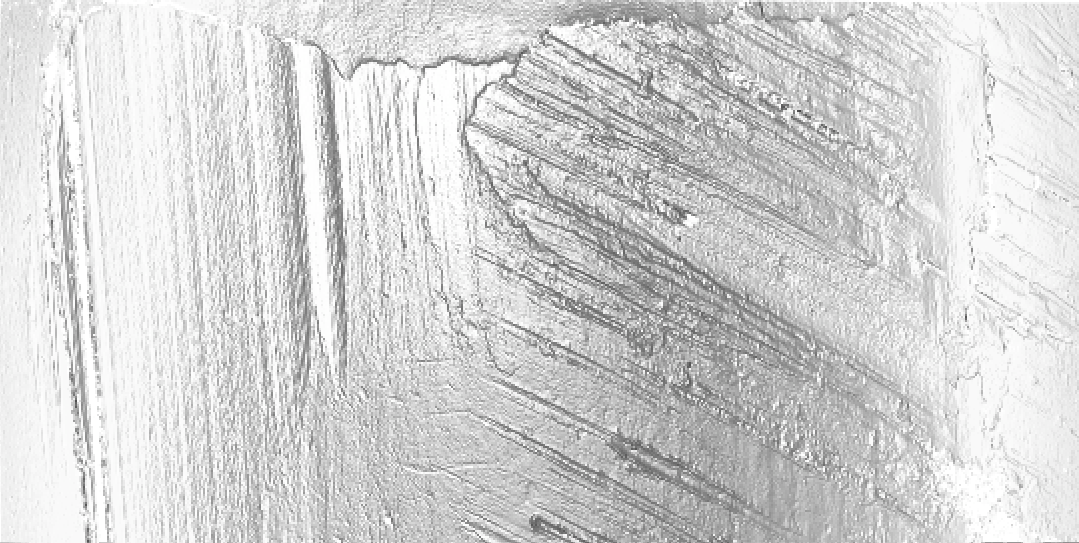
\includegraphics[width=\linewidth]{images/br9-2-4-greyflip.png}
\caption{Land 4 of Bullet 2, from Barrel 9 of Hamby Set 252. It can be seen that this particular land exhibits some major tank rash on the right half.}
\label{fig:br924}
\end{figure}

Table \ref{tab:br924pred} shows the values of the features, after
extracting only the first 50\% of the Hamby Barrel 9 Bullet 2, 4th land
(and hence, simulating a left-fixed 50\% degraded scenario), compared
with a feature comparison between both full lands (and hence, including
the tank rash striae). The features are derived in a comparison with its
known match, the complete Bullet 1 third land fired from Barrel 9. The
features, including the ccf and the matches, are expressed enough to
(barely) indicate a match in the case of the degraded bullet. Using the
pre-trained random forest, the predicted matching probability is 52\%.
This is encouraging in that attempting to match the full bullet land, by
comparison, yields a matching probability of 0.0067\%. This is due to
the relatively higher values of the ccf, cms, and matches for the
degraded comparison, and suggests that the feature standardization is
working as intended.

\begin{table}[ht]
\centering
\begin{tabular}{lrr}
  \hline
Feature & Degraded Land & Full Land \\ 
  \hline
ccf & 0.6004 & 0.4442 \\ 
  rough\_cor & 0.3671 & 0.1633 \\ 
  D & 0.0018 & 0.0023 \\ 
  overlap & 0.9968 & 0.9968 \\ 
  matches & 10.2236 & 5.6275 \\ 
  mismatches & 7.5949 & 5.0713 \\ 
  cms & 9.2013 & 4.6043 \\ 
  non\_cms & 6.5823 & 2.5357 \\ 
  sum\_peaks & 12.0020 & 6.3148 \\ 
  matchprob & 0.5200 & 0.0067 \\ 
   \hline
\end{tabular}
\caption{Features extracted for a comparison of the full Hamby Barrel 9 Bullet 1 Land 3, with a left-fixed 50 percent degraded portion of Hamby Barrel 9 Bullet 2 Land 4. These two lands are known matches, and indeed the random forest does predict a match.} 
\label{tab:br924pred}
\end{table}

\addtocontents{toc}{\protect\newpage}

\section{From Lands to Bullets}\label{from-lands-to-bullets}

Another area that deserves more study is the question of generalizing
these algorithms to matching entire bullets rather than indvidual lands,
as would be done in a criminal justice application. One such approach is
to recognize that (at least for the Hamby bullets) there should be six
matching pairs of lands for any two bullets that were fired from the
same gun barrel. Therefore, for each pair of bullets, we can extract the
six highest matching probabilities and average them. If we do so, we
obtain a clear separation between the scores that are obtained when
matching bullets known to be matches and the scores obtained from known
non-matches. This is shown in Figure \ref{fig:firstscore}. No
known-matches have a score below 50\%, while all known non-matches have
a score below 10\%.

We can improve on this approach by exploiting the rotation of the bullet
to compute a score. Under the assumption of land to land independence,
we can define the probability that two bullets match (M) as one minus
the probability that the two bullets do not match (NM). Exploiting the
idea that when two bullets do not match, none of the individual lands
match either, we can write the matching probability as the probability
that at least one land pair in the matrix matches. Specifically,

\begin{align}
P(M) &= 1 - P(NM) \\
     &= 1 - (P(NM1) \times P(NM2) \times ... \times P(NM6)) \\
     &= 1 - ((1 - P(M1)) \times (1 - P(M2)) \times ... \times (1 - P(M6)))
\end{align}

Where \(M\) is the event that two bullets match, \(NM\) is the event
that two bullets do not match, \(M1\), \(M2\), \ldots{}, \(M6\) are the
probabilities of land one, land two, \ldots{}, land six matching, and
\(NM1\), \(NM2\), \ldots{}, \(NM6\) are the probabilities that land one,
land two, \ldots{}, land six do not match. However, to compute this
probability, we need to know the alignment of the two sets of lands.
Fortunately, the consistent rotation of the bullet permits this. For
instance, if we knew that land 1 of bullet 1 matches land 4 of bullet 2,
then we immediately know that land 2 of bullet 1 matches to land 5 of
bullet 2, land 3 of bullet 1 matches to land 6 of bullet 2, etc. Hence,
we can take look across six diagonals of the \(6 \otimes 6\) matrix
containing match probabilities. Table \ref{tab:diag} gives an example of
the matrix of matching probabilities between two sets of six lands from
bullets that are known matches. The matching diagonal is clear based on
the high probabilities (cell \((1, 3)\), cell \((2, 4)\), cell
\((3, 5)\), etc.) although it can be seen that one of the six
comparisons has a relatively lower matching probability. This procedure
is based on the Sequence Average Maximum (SAM) by Sensorfar (2017) in
their bullet matching software application \texttt{SensoMatch}.

\begin{table}[ht]
\centering
\begin{tabular}{rrrrrrr}
  \hline
profile1\_id & 45604 & 46104 & 46601 & 47069 & 47600 & 48069 \\ 
  \hline
42594 & 0.0000 & 0.0000 & 1.0000 & 0.0000 & 0.0000 & 0.0000 \\ 
  43063 & 0.0000 & 0.0000 & 0.0000 & 1.0000 & 0.0067 & 0.0000 \\ 
  43581 & 0.0000 & 0.0000 & 0.0000 & 0.0000 & 0.8433 & 0.0000 \\ 
  44211 & 0.0000 & 0.0000 & 0.0133 & 0.0000 & 0.0000 & 0.6700 \\ 
  44568 & 1.0000 & 0.0000 & 0.0033 & 0.0000 & 0.0000 & 0.0000 \\ 
  45070 & 0.0000 & 1.0000 & 0.0000 & 0.0000 & 0.0000 & 0.0000 \\ 
   \hline
\end{tabular}
\caption{Matrix of matching probabilities between two sets of six lands from bullets that are known matches.} 
\label{tab:diag}
\end{table}

We derive a score by computing the bullet matching probability on each
set of six matrix diagonals using the previously defined formula, under
the assumption of land to land indepndence. Finally, we take the maximum
score obtained out of the six results as the final matching score for a
bullet pair. After doing so, we can plot the scores for known matches
and known non-matches separately. Figure \ref{fig:scores} provides the
distribution of matching scores for known matches compared to known
non-matches. It can be seen that the known matches all have scores of
around 100\%, while no non-match achieves a score of above 30\%, and
hence this procedure provides perfect discrimination between all pairs
of bullets between and within the two Hamby datasets.

\begin{figure}[htbp]
\centering
\includegraphics{degraded-paper_files/figure-latex/scores-1.pdf}
\caption{\label{fig:scores}Distribution of matching scores for known matches
compared to known non-matches. It can be seen that the known matches all
have scores of around 100\%, while no non-match achieves a score of
above 30\%.}
\end{figure}

On the other hand, flipping this procedure around by assuming that a
match occurs if and only if all six lands match does not discriminate
quite as well, as can be seen in Figure \ref{fig:scores1}. Every known
bullet non-match achieves a score of about zero, but so do about 15
known bullet matches. This method performs poorly because our matching
algorithm exhibits a larger false negative rate than the rate of false
positives. Multiplying the probabilities together compounds the issue of
false negatives and leads to some misidentification of matching bullets.

\begin{figure}[htbp]
\centering
\includegraphics{degraded-paper_files/figure-latex/scores1-1.pdf}
\caption{\label{fig:scores1}Distribution of matching scores for known
matches compared to known non-matches when assuming a match occurs if
and only if all six lands match. Now, it can be seen that the known
non-matches all have scores of around 0, while most though not all known
matches achieve much higher scores.}
\end{figure}

If we construct a hybrid of these two approaches, we can average the
probabilities along the diagonal rather than multiplying those
probabilities. Doing so yields the distributions shown in Figure
\ref{fig:scores10}. Now, we once again differentiate the two groups well
with no known non-match achieving a score above 10\%, and no known match
with a score below 40\%.

\begin{figure}[htbp]
\centering
\includegraphics{degraded-paper_files/figure-latex/scores10-1.pdf}
\caption{\label{fig:scores10}Distribution of matching scores for known
matches compared to known non-matches obtained by averaging the
probabilities along the maximal diagonal. Once again, it can be seen
that the known non-matches all have scores of around 0, but the known
matches this time are well separated, with nearly all achieving scores
above .5.}
\end{figure}

One more approach to match bullets would exploit the SAM procedure on
individual features. For each diagonal in the \(6 \otimes 6\) matrix, we
can compute an average value for each feature in our model. This yields
six sets of feature values for all six diagonals. We can then feed all
six sets of features into the random forest in order to obtain a
matching probability for each, taking the highest resulting probability
to locate the diagonal and thus identify land to land alignment. Figure
\ref{fig:scores2} shows boxplots of the matching scores using this
hybrid procedure. It can be seen that while this procedure does
discriminate well, it yields some false negatives (matching bullets that
our forest identifies as a non-match).

\begin{figure}[htbp]
\centering
\includegraphics{degraded-paper_files/figure-latex/scores2-1.pdf}
\caption{\label{fig:scores2}Distribution of matching scores using a SAM
procedure on the feature values for known matches compared to known
non-matches.}
\end{figure}

\section{Conclusion}\label{conclusion}

In this paper, we have introduced a set of robust features that can be
used to train bullet matching models. We have used these features to
train a random forest and assess its out-of-sample accuracy. In doing
so, we noted strong evidence of operator effects that resulted in
differences in the quality of the microscope scans.

While these effects were clearly identified, the best approach to
account for them in practice is less clear. In the ideal case, bullets
fired from a particular gun barrel should yield surface scans that are
of identical quality and properties, regardless of the operator
performing the scan. To achieve this, rigorous standards may need to be
put in place with regards to the alignment of the bullet under the
objective, and the procedure used to scan the bullet surface. To
appropriately design a set of best practices requires more research. For
instance, because of the significant difference between the placement of
the ideal cross section across the two studies, a best practice may
specify the margin from the edge of the objective at which the bullet
can be placed.

We begain exploring the robustness of the matching algorithm proposed in
(Hare, Hofmann, and Carriquiry 2016) to land degradation. As suspected,
the algorithm performance declines as a function of the rate of
degradation. However, there is a relatively clear threshold around about
50\%; if 50\% of the land or more is recovered, the algorithm still
performs reasonably well. When the proportion of the land that is
recovered is below 50\%, the accuracy with which we can compare land
impressions is low.

As we have stated before, the lack of 3D images of bullets limits the
extent to which these algorithms can be tested and validated. The
degraded land simulation itself may be too simplistic and not faithfully
represent realistic scenarios. However, as more data are collected, we
can continue to update, train and test the matching algorithm in order
to improve its performance in real datasets.

\clearpage

\section{Appendix}\label{appendix}

\begin{table}[ht]
\centering
\begin{tabular}{llllrlr}
  \hline
set1 & set2 & feature & matchtest & matchd & nonmatchtest & nonmatchd \\ 
  \hline
H252\_H252 & H252\_H44 & ccf & $<$ 0.0001 & 0.2723 & 1e-04 & 0.0189 \\ 
  H252\_H252 & H252\_H44 & cms & $<$ 0.0001 & 0.1751 & $<$ 0.0001 & 0.0245 \\ 
  H252\_H252 & H252\_H44 & D & $<$ 0.0001 & 0.2567 & $<$ 0.0001 & 0.1049 \\ 
  H252\_H252 & H252\_H44 & matches & $<$ 0.0001 & 0.1933 & $<$ 0.0001 & 0.0327 \\ 
  H252\_H252 & H252\_H44 & mismatches & $<$ 0.0001 & 0.2015 & 0.3537 & 0.0079 \\ 
  H252\_H252 & H252\_H44 & overlap & 0.0492 & 0.0984 & $<$ 0.0001 & 0.0276 \\ 
  H252\_H252 & H252\_H44 & rough\_cor & $<$ 0.0001 & 0.2647 & $<$ 0.0001 & 0.0970 \\ 
  H252\_H252 & H252\_H44 & sum\_peaks & 8e-04 & 0.1426 & 0.0015 & 0.0162 \\ 
  H252\_H252 & H44\_H44 & ccf & $<$ 0.0001 & 0.2160 & $<$ 0.0001 & 0.0257 \\ 
  H252\_H252 & H44\_H44 & cms & $<$ 0.0001 & 0.2515 & $<$ 0.0001 & 0.0467 \\ 
  H252\_H252 & H44\_H44 & D & $<$ 0.0001 & 0.2342 & $<$ 0.0001 & 0.1946 \\ 
  H252\_H252 & H44\_H44 & matches & $<$ 0.0001 & 0.2770 & $<$ 0.0001 & 0.0713 \\ 
  H252\_H252 & H44\_H44 & mismatches & $<$ 0.0001 & 0.2505 & 0.0414 & 0.0138 \\ 
  H252\_H252 & H44\_H44 & overlap & 0.2432 & 0.0906 & $<$ 0.0001 & 0.0408 \\ 
  H252\_H252 & H44\_H44 & rough\_cor & $<$ 0.0001 & 0.2242 & $<$ 0.0001 & 0.1718 \\ 
  H252\_H252 & H44\_H44 & sum\_peaks & 1e-04 & 0.1926 & $<$ 0.0001 & 0.0289 \\ 
  H252\_H44 & H44\_H44 & ccf & 0.1149 & 0.0883 & $<$ 0.0001 & 0.0259 \\ 
  H252\_H44 & H44\_H44 & cms & 0.111 & 0.0888 & $<$ 0.0001 & 0.0262 \\ 
  H252\_H44 & H44\_H44 & D & 0.2923 & 0.0724 & $<$ 0.0001 & 0.0906 \\ 
  H252\_H44 & H44\_H44 & matches & 0.0603 & 0.0977 & $<$ 0.0001 & 0.0423 \\ 
  H252\_H44 & H44\_H44 & mismatches & 0.3301 & 0.0700 & 0.1633 & 0.0096 \\ 
  H252\_H44 & H44\_H44 & overlap & 0.8231 & 0.0465 & 1e-04 & 0.0190 \\ 
  H252\_H44 & H44\_H44 & rough\_cor & 0.2671 & 0.0741 & $<$ 0.0001 & 0.0769 \\ 
  H252\_H44 & H44\_H44 & sum\_peaks & 0.047 & 0.1011 & 0.006 & 0.0147 \\ 
   \hline
\end{tabular}
\caption{Results for the Kolmogrov-Smirnov distributional test.} 
\label{tab:kstests}
\end{table}

\begin{figure}[htbp]
\centering
\includegraphics{degraded-paper_files/figure-latex/deghist-1.pdf}
\caption{\label{fig:deghist}Histograms of matching probability, facetted by
the degradation level and known match versus known non-match.}
\end{figure}

\begin{figure}[htbp]
\centering
\includegraphics{degraded-paper_files/figure-latex/firstscore-1.pdf}
\caption{\label{fig:firstscore}Score distributions for the naive approach to
bullet matching, for known matches and known non-matches.}
\end{figure}

\hypertarget{refs}{}
\hypertarget{ref-pcast2016}{}
Advisors on Science, President's Council of, and Technology. 2016.
``Report on Forensic Science in Criminal Courts: Ensuring Scientific
Validity of Feature-Comparison Methods.''
\url{https://www.whitehouse.gov/sites/default/files/microsites/ostp/PCAST/pcast_forensic_science_report_final.pdf}.

\hypertarget{ref-biasotti:1959}{}
Biasotti, Alfred A. 1959. ``A Statistical Study of the Individual
Characteristics of Fired Bullets.'' \emph{Journal of Forensic Sciences}
4 (1): 34--50.

\hypertarget{ref-chu:2011}{}
Chu, W., J. Song, T. Vorburger, R. Thompson, and R. Silver. 2011.
``Selecting Valid Correlation Areas for Automated Bullet Identification
System Based on Striation Detection.'' \emph{Journal of Research of the
National Institute of Standards and Technology} 116 (3): 649.

\hypertarget{ref-thompson:2013}{}
Chu, Wei, Robert M Thompson, John Song, and Theodore V Vorburger. 2013.
``Automatic identification of bullet signatures based on consecutive
matching striae (CMS) criteria.'' \emph{Forensic Science International}
231 (1--3): 137--41.

\hypertarget{ref-clarkson1933definitions}{}
Clarkson, James A, and C Raymond Adams. 1933. ``On Definitions of
Bounded Variation for Functions of Two Variables.'' \emph{Transactions
of the American Mathematical Society} 35 (4). JSTOR: 824--54.

\hypertarget{ref-giannelli:2011}{}
Giannelli, Paul C. 2011. ``Ballistics Evidence Under Fire.''
\emph{Criminal Justice} 25 (4): 50--51.

\hypertarget{ref-hamby:2009}{}
Hamby, James E., David J. Brundage, and James W. Thorpe. 2009. ``The
Identification of Bullets Fired from 10 Consecutively Rifled 9mm Ruger
Pistol Barrels: A Research Project Involving 507 Participants from 20
Countries.'' \emph{AFTE Journal} 41 (2): 99--110.

\hypertarget{ref-2016arXiv160105788H}{}
Hare, E., H. Hofmann, and A. Carriquiry. 2016. ``Automatic Matching of
Bullet Lands.'' \emph{ArXiv E-Prints}, January.

\hypertarget{ref-caretpkg}{}
Jed Wing, Max Kuhn. Contributions from, Steve Weston, Andre Williams,
Chris Keefer, Allan Engelhardt, Tony Cooper, Zachary Mayer, et al. 2016.
\emph{Caret: Classification and Regression Training}.
\url{https://CRAN.R-project.org/package=caret}.

\hypertarget{ref-randomForest}{}
Liaw, Andy, and Matthew Wiener. 2002. ``Classification and Regression by
RandomForest.'' \emph{R News} 2 (3): 18--22.
\url{http://CRAN.R-project.org/doc/Rnews/}.

\hypertarget{ref-NAS:2009}{}
National Research Council. 2009. \emph{Strengthening Forensic Science in
the United States: A Path Forward}. Washington, DC: The National
Academies Press.
doi:\href{https://doi.org/10.17226/12589}{10.17226/12589}.

\hypertarget{ref-petraco:2012}{}
Petraco, Nicholas, and Helen Chan. 2012. \emph{Application of Machine
Learning to Toolmarks: Statistically Based Methods for Impression
Pattern Comparisons}. Mannheim, Germany: Bibliographisches Institut AG.

\hypertarget{ref-riva:2014}{}
Riva, Fabiano, and Christophe Champod. 2014. ``Automatic Comparison and
Evaluation of Impressions Left by a Firearm on Fired Cartridge Cases.''
\emph{Journal of Forensic Sciences} 59 (3): 637--47.
doi:\href{https://doi.org/10.1111/1556-4029.12382}{10.1111/1556-4029.12382}.

\hypertarget{ref-sensorfar}{}
Sensorfar. 2017. \emph{SensoMATCH Bullet Comparison Software}.

\hypertarget{ref-vorburger:2011}{}
Vorburger, T.V., J.-F. Song, W. Chu, L. Ma, S.H. Bui, A. Zheng, and T.B.
Renegar. 2011. ``Applications of Cross-Correlation Functions.''
\emph{Wear} 271 (3--4): 529--33.
doi:\href{https://doi.org/http://dx.doi.org/10.1016/j.wear.2010.03.030}{http://dx.doi.org/10.1016/j.wear.2010.03.030}.


\end{document}
